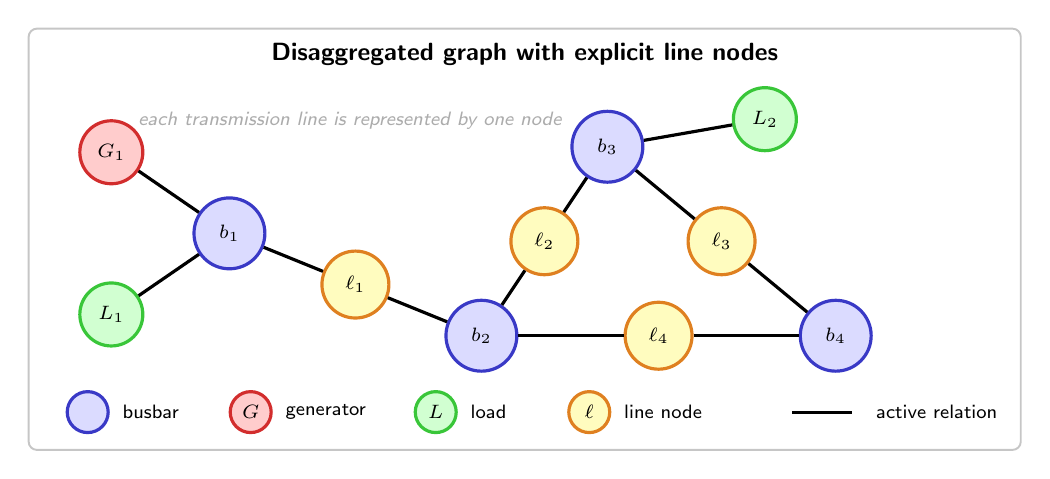
\begin{tikzpicture}[
  x=1cm,
  y=1cm,
  font=\sffamily,
  busbar/.style={
    circle,
    draw=blue!55!gray,
    fill=blue!14,
    line width=1.15pt,
    minimum size=9mm,
    inner sep=0pt,
    font=\scriptsize\sffamily
  },
  generator/.style={
    circle,
    draw=red!65!gray,
    fill=red!20,
    line width=1.15pt,
    minimum size=8mm,
    inner sep=0pt,
    font=\scriptsize\sffamily
  },
  load/.style={
    circle,
    draw=green!55!gray,
    fill=green!18,
    line width=1.15pt,
    minimum size=8mm,
    inner sep=0pt,
    font=\scriptsize\sffamily
  },
  linenode/.style={
    circle,
    draw=orange!75!gray,
    fill=yellow!25,
    line width=1.15pt,
    minimum size=8.5mm,
    inner sep=0pt,
    font=\scriptsize\sffamily
  },
  physical/.style={draw=black, line width=1.15pt},
  panel/.style={draw=gray!45, rounded corners=3pt, line width=0.7pt},
  title/.style={font=\small\bfseries\sffamily},
  note/.style={font=\scriptsize\sffamily, align=center},
  muted/.style={font=\scriptsize\itshape\sffamily, align=center, text=gray!65}
]

\path[panel] (0,0) rectangle (12.6,5.35);
\node[title] at (6.3,5.02) {Disaggregated graph with explicit line nodes};

\node[busbar] (b1) at (2.55,2.75) {$b_1$};
\node[busbar] (b2) at (5.75,1.45) {$b_2$};
\node[busbar] (b3) at (7.35,3.85) {$b_3$};
\node[busbar] (b4) at (10.25,1.45) {$b_4$};
\node[generator] (g1) at (1.05,3.78) {$G_1$};
\node[load] (d1) at (1.05,1.72) {$L_1$};
\node[load] (d2) at (9.35,4.20) {$L_2$};

\node[linenode] (l12) at (4.15,2.10) {$\ell_1$};
\node[linenode] (l23) at (6.55,2.65) {$\ell_2$};
\node[linenode] (l34) at (8.80,2.65) {$\ell_3$};
\node[linenode] (l24) at (8.00,1.45) {$\ell_4$};

\draw[physical] (g1) -- (b1);
\draw[physical] (d1) -- (b1);
\draw[physical] (d2) -- (b3);
\draw[physical] (b1) -- (l12) -- (b2);
\draw[physical] (b2) -- (l23) -- (b3);
\draw[physical] (b3) -- (l34) -- (b4);
\draw[physical] (b2) -- (l24) -- (b4);

\node[muted] at (4.08,4.18)
  {each transmission line is represented by one node};

% Compact legend.
\node[busbar, minimum size=5.2mm] at (0.75,0.48) {};
\node[note, anchor=west] at (1.07,0.48) {busbar};
\node[generator, minimum size=5.2mm] at (2.82,0.48) {$G$};
\node[note, anchor=west] at (3.14,0.48) {generator};
\node[load, minimum size=5.2mm] at (5.17,0.48) {$L$};
\node[note, anchor=west] at (5.49,0.48) {load};
\node[linenode, minimum size=5.2mm] at (7.12,0.48) {$\ell$};
\node[note, anchor=west] at (7.44,0.48) {line node};
\draw[physical] (9.70,0.48) -- (10.46,0.48);
\node[note, anchor=west] at (10.64,0.48) {active relation};

\end{tikzpicture}
